\chapter{Method} \label{ch:method}
%\Conventional method using calorimeters
%\ first the math: definitions 1.3, 1.4 from analysis note
%\ then the description of the instruments used to get the relevant variables:
%\ 		primarily STAR (reference 12 from analysis note), include PHENIX and CMS later if needed

%\ transition to:

%\Spectra from the BES program
%\ Beam Energy Scan program
%\ particle identification
%\ transverse momentum spectrum (using tracking detectors????)
%\ errors associated with the spectra

%\Getting ET estimates from the spectra for individual particles
%\ equations relating dET/dy etc. to the pT integral of d2N/(dydpT)
%\ extrapolation of spectra to cover regions not covered by the experiment
%\ using ET estimates for individual particles to estimate total ET and the assumptions involved
%\ analysis note pg 7: "In this new method, ET is measured from charged hardon tracks...
%\ and the measured ET is SCALED UP to correct for neutral energy which is not observed...
%\ in tracking detectors."
%\ essentially, what really needs to be made clear is how the "scaling up" is done, because...
%\ even conventionally, STAR "uses information from the tracking detectors to measure ET from...
%\ charged hadrons and the electromagnetic calorimeter to measure ET from electrons, photons...
%\ and neutral hadrons which dominantly decay to electromagnetic particles." (hybrid method)

%\ centrality determination
In theory, $E_{T}$ from a collision can be defined as the sum of the transverse masses, $m_{T}$, of all the particles produced in the collision, i.e.,
\begin{equation}\label{eqn:ETDefTheory}
E_{T}\equiv\sum_{i}m_{T,i}
\end{equation}
with
\begin{equation}\label{eqn:mT}
m_{T}\equiv\sqrt{p_{T}^{2}+m^2}
\end{equation}
where $m$ is the rest mass of the particle and $p_{T}$ is its transverse momentum. Using this definition to calculate the $E_{T}$ requires perfect identification of all the particles. It has not been possible to do so in experiments, and so a more feasible, operational definition of $E_{T}$ is fabricated. A commonly accepted definition in case of the feasibility of calorimetric measurements is \cite{PhysRevC.89.044905, PhysRevLett.109.152303}:
\begin{equation}\label{eqn:ETDefSum}
E_{T} = \sum_{i}E_{i}\sin{\theta_{i}},
\end{equation}
\begin{equation}\label{eqn:dETdEta}
\frac{dE_{T}}{d\eta}=\sin{\theta}\frac{dE}{d\eta},
\end{equation}

where the index $i$ runs over all the particles going into a fixed solid angle for each event, $\theta$ is the polar angle, i.e, the angle with respect to the beam axis, $\eta$ is the pseudorapidity defined as 
\begin{equation}\label{eqn:pseudorap}
\eta\equiv-\ln\tan{\frac{\theta}{2}},
\end{equation}
and $E_{i}$ is the energy deposited in the calorimeter by the $i^{th}$ particle. $E_{i}$ is considered to be, by convention \cite{PhysRevC.71.034908}, the following
\begin{equation}\label{eqn:EiCaseByCase}
E_{i} = 
	\begin{cases}
	E_{i}^{tot}-m_{0} & \text{for baryons} \\
	E_{i}^{tot}+m_{0} & \text{for anti-baryons} \\	
	E_{i}^{tot} & \text{otherwise} \\
	\end{cases}
\end{equation}
%\ $E_{i}^{tot}$ - $m_{N}$ in case of baryons, $E_{i}^{tot}$ + $m_{N}$ in case of antibaryons, and the $E_{i}^{tot}$ in case of other particles, 
where $E_{i}^{tot}$ is the total energy of the $i^{th}$ particle defined canonically as
\begin{equation}\label{eqn:Etot}
E^{tot}\equiv\sqrt{p^{2}+m_{0}^2}
\end{equation}
and  $m_{0}$ is the particle's rest mass.
In order to account for the portion of the emitted transverse energy not detected or overestimated by the calorimeters, corrections are made based on GEANT simulations.
%\ split the following into a sub-chapter
Transverse energy analysis can be done using tracking detectors as well if they are able to produce measurements of other physical quantities that implicitly contain information about the transverse energy. Specifically, the charged particle multiplicity distributions with respect to the transverse momenta can be used to calculate the particle's transverse energy pseudorapidity density. In fact, since the corrections related to the tracking detectors are very different from those related to the calorimeters, results from the two different methods can be used to test the assumptions involved in each.

The tracking detectors in experiments such as the STAR (Solenoidal Tracker At RHIC) experiment and ALICE (A Large Ion Collider Experiment) at CERN include Time Projection Chambers (TPCs) and Time-of-Flight (TOF) detectors that can give us the $p_{T}$ spectra, yields and particle ratios of the identified charged hadrons \cite{Preghenella:2011vy, PhysRevC.96.044904}. The TPCs provide measurements of particle trajectories -- that can be used to determine the momenta for low-momentum particles -- and of their specific energy loss, 
\begin{equation}\label{eqn:specificEnLoss}
	\frac{dE}{dx} ,
\end{equation}
which can be used with the trajectories to make particle identifications using the Bethe-Bloch formula \cite{bethe1953passage}. TOF detectors, on the other hand, cover the high-momentum part of the measurements. In ALICE, the combination of the measurements of the TPC with those of the Inner Tracking System (ITS) effectively adds the tracking length, thereby improving the resolution of the measured $p_{T}$ spectrum. Details about the particle identification and momentum determination capabilities of the detectors in ALICE can be found in \cite{1748-0221-3-08-S08002}.

In the STAR experiment, the TPC is the primary tracking detector. It is 4.2 m long and it cylindrically enshrouds the accelerator beam pipe from its outside, with an inner diameter of 1 m and an outer diameter of 4 m \cite{phdthesisnattrass}. !!!!!!!!!........ more details about the TPC, then its limitation in high momentum resolution, then transition to TOF and some of its details ..........!!!!!!!!!
%\Its drift volume is full of P10 gas (10% methane and 90% argon), the electrons from the molecules of which are knocked off by a charged particle travelling through the medium.

%\Spectra from the BES program (PhysRevC.96.044904 : https://arxiv.org/pdf/1701.07065.pdf)
%\ Beam Energy Scan program
%\ particle identification
%\ transverse momentum spectrum (using tracking detectors????)
%\ errors associated with the spectra

The RHIC, in 2010, started a multi-phase Beam Energy Scan (BES) program to study the QCD phase diagram. The collider has the unique facility to collide nulclei at a range of center-of-mass energies per nucleon, $\sqrt{s_{NN}}$. It also has two different detectors that are currently operational, STAR and PHENIX (Pioneering High Energy Nuclear Interactions eXperiment), which facilitate the cross-checking of results. Between 2010 and 2011, under the exploratory phase I of the BES program, 7.7, 11.5 (not completed in PHENIX), 19.6, 27, and 39 GeV collisions were completed using pairs of Au nuclei. Together with the data formerly collected by the RHIC at higher collision energies, BES phase I data can scan the interval from 450 MeV to 20 MeV in $\mu_{B}$ space \cite{1742-6596-455-1-012037, LUO201675}. One of the things that can be studied with the data associated with this region of the phase space is statedly the possibility of a ``turn-off of new phenomena already established at higher RHIC energies" (https://drupal.star.bnl.gov/STAR/starnotes/public/sn0493). Results corresponding to the high-$\mu_{B}$ region might provide evidence of a first order phase transition, and possibly the critical point \cite{LUO201675}.

The manifestation of such phenomena would be in terms of the fluctuations in the properties of the post-collision system. One can, for instance, study the scaling of the transverse energy after the collision with the longidutional energy at the time of the collision, $\sqrt{s_{NN}}$. This can be done in multiple ways for a detector like STAR or PHENIX that is made up of sub-systems such as the TOF detectors, TPCs/Time Expansion Chambers, and calorimeters. 

\citet{PhysRevC.93.024901} use calorimetry in PHENIX to analyze the transverse energy corresponding to several different pairs of species colliding at a range of energies. They use the raw transverse energy measured by the EMCal, $E_{{T}EMC}$, to obtain the total hadronic $E_{T}$ by making corrections in three different steps. They first scale the data by a constant factor calculated to account for the fiducial acceptance in azimuth and pseudorapidity. The second factor is calculated to adjust for the effects of the calorimeter towers that are disabled. The third factor, $k$, is computed as follows
\begin{equation}\label{eqn:AdareKfactor}
k = k_{response} \times k_{inflow} \times k_{losses}
\end{equation}
where $k_{response}$ corresponds to hadronic particles only depositing a fraction of their total energy while passing through the EMCal, $k_{inflow}$ is attributable to the energy deposited by particles coming from outside the EMCal's fiducial aperture, and $k_{losses}$ accounts for the energy not registered in the EMCal due to energy thresholds, edge effects, and more importantly due to the particles that make it into the fiducial aperture but decay into products outside the aperture.

Another method of transverse energy analysis, employed in this thesis, is to use the $p_{T}$ spectra available from the tracking detectors. The TPCs and TOF detectors in STAR, for instance, can identify particles as well as their trajectories and ultimately their multiplicity distributions with respect to the momenta. \citet{PhysRevC.96.044904} report the results for the $p_{T}$ spectra for six different identified hadrons, $\pi^+$, $\pi^-$, $K^+$, $K^-$, $p$, and $\bar{p}$, from the STAR experiment. The spectra come from Au+Au collisions -- at $\sqrt{s_{NN}}$ = 7.7, 11.5, and 39 GeV in the year 2010 and at $\sqrt{s_{NN}}$ = 19.6 and 27 GeV in 2011 -- under the BES Program. Figure \ref{fig:BESPaper_pTSpectra} \cite{PhysRevC.96.044904} shows the spectra corresponding to 39 GeV collisions categorized into seven different collision centralitiy classes. These spectra, and their counterparts for the rest of the energies, were used to calculate an estimate of the total transverse energy per event per particle species. This result was then used to estimate the total transverse energy due to all the collision products. The corrections applied by \citet{PhysRevC.96.044904} to the raw data to obtain the spectra, the reported systematic uncertainties in their results, and the mathematics involved in calculating the transverse energy results using the $p_{T}$ spectra are discussed below.
\begin{figure}[h]
  \centering
  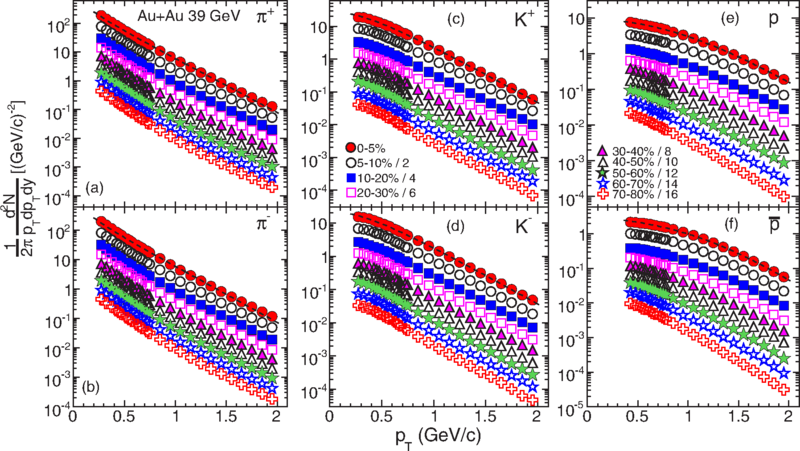
\includegraphics[width=5.5in]{../figures/PhysRevC-96-044904_pTSpectra_39.png}\\
  \caption{Transverse momentum spectra for $\pi^{+}$, $\pi^{-}$, $K^+$, $K^{-}$, $p$, and $\bar{p}$ at midrapidity ($|y|$ $<$ 0.1) from 39 GeV Au+Au collisions at RHIC. The fitting curves on the 0-5\% central collision spectra for pions, kaons, and protons/anti-protons represent, respectively, the Bose-Einstein, $m_{T}$-exponential, and double-exponential functions. \cite{PhysRevC.96.044904}.}\label{fig:BESPaper_pTSpectra}
\end{figure}
%...... mathematics involved in getting ET out of pT spectra, including the extrapolation using the BGBW.............

%...... assumption leading to total ET estimate, i.e, how the scaling up is done, and the errors associated with it...............

%chapter 3: data analysis
%go through the steps from getting the data to getting the final results
%example fit plots
%justification of using chi-squared

%chapter 4: results
%plots and tables compared to what's been published.
%Anything interesting seen?

%chapter 5: conclusion
%chapter 6: future work

%acknowledgments
%christine, adam, charles, soren, andy, will, chrisanne.
%\ NEXT: WRITE ABOUT THE ALTERNATIVE WAY, THAT IS, USING SPECTRA, AND WHAT DETECTOR THIS METHOD USES INSTEAD


%\"The main detectors used to obtain the results on pT spectra, yields and particle ratios for charged hadrons are the Time Projection Chamber (TPC) [41] and Time-Of Flight detectors (TOF) [42]" https://arxiv.org/pdf/1701.07065.pdf
%\ " The TPC data is used to determine particle trajectories, thereby their momenta, and particle types through ionization energy loss (dE/dx)."
%\ "For higher momentum, we use time-of-flight information to identify particles. The TOF particle identification for this analysis is used above pT = 0.4 GeV/c."

%\Historically, measurement of $E_{T}$ would be one of the first things done after heavy-ion collisions. Electromagnetic calorimeters (EMCals) would be used to perform the measurement of $E_{T}$. 
